\documentclass[]{book}
\usepackage{lmodern}
\usepackage{setspace}
\setstretch{2}
\usepackage{amssymb,amsmath}
\usepackage{ifxetex,ifluatex}
\usepackage{fixltx2e} % provides \textsubscript
\ifnum 0\ifxetex 1\fi\ifluatex 1\fi=0 % if pdftex
  \usepackage[T1]{fontenc}
  \usepackage[utf8]{inputenc}
\else % if luatex or xelatex
  \ifxetex
    \usepackage{mathspec}
  \else
    \usepackage{fontspec}
  \fi
  \defaultfontfeatures{Ligatures=TeX,Scale=MatchLowercase}
    \setmainfont[]{FreeSerif}
\fi
% use upquote if available, for straight quotes in verbatim environments
\IfFileExists{upquote.sty}{\usepackage{upquote}}{}
% use microtype if available
\IfFileExists{microtype.sty}{%
\usepackage{microtype}
\UseMicrotypeSet[protrusion]{basicmath} % disable protrusion for tt fonts
}{}
\usepackage[margin=1in]{geometry}
\usepackage{hyperref}
\hypersetup{unicode=true,
            pdftitle={Knowledge of the U.S. Social Sciences, 1888--1922},
            pdfauthor={Brooks Ambrose},
            pdfborder={0 0 0},
            breaklinks=true}
\urlstyle{same}  % don't use monospace font for urls
\usepackage{natbib}
\bibliographystyle{apalike}
\usepackage{longtable,booktabs}
\usepackage{graphicx,grffile}
\makeatletter
\def\maxwidth{\ifdim\Gin@nat@width>\linewidth\linewidth\else\Gin@nat@width\fi}
\def\maxheight{\ifdim\Gin@nat@height>\textheight\textheight\else\Gin@nat@height\fi}
\makeatother
% Scale images if necessary, so that they will not overflow the page
% margins by default, and it is still possible to overwrite the defaults
% using explicit options in \includegraphics[width, height, ...]{}
\setkeys{Gin}{width=\maxwidth,height=\maxheight,keepaspectratio}
\setlength{\emergencystretch}{3em}  % prevent overfull lines
\providecommand{\tightlist}{%
  \setlength{\itemsep}{0pt}\setlength{\parskip}{0pt}}
\setcounter{secnumdepth}{5}
% Redefines (sub)paragraphs to behave more like sections
\ifx\paragraph\undefined\else
\let\oldparagraph\paragraph
\renewcommand{\paragraph}[1]{\oldparagraph{#1}\mbox{}}
\fi
\ifx\subparagraph\undefined\else
\let\oldsubparagraph\subparagraph
\renewcommand{\subparagraph}[1]{\oldsubparagraph{#1}\mbox{}}
\fi

%%% Use protect on footnotes to avoid problems with footnotes in titles
\let\rmarkdownfootnote\footnote%
\def\footnote{\protect\rmarkdownfootnote}

%%% Change title format to be more compact
\usepackage{titling}

% Create subtitle command for use in maketitle
\newcommand{\subtitle}[1]{
  \posttitle{
    \begin{center}\large#1\end{center}
    }
}

\setlength{\droptitle}{-2em}

  \title{Knowledge of the U.S. Social Sciences, 1888--1922}
    \pretitle{\vspace{\droptitle}\centering\huge}
  \posttitle{\par}
    \author{Brooks Ambrose}
    \preauthor{\centering\large\emph}
  \postauthor{\par}
      \predate{\centering\large\emph}
  \postdate{\par}
    \date{2018-11-14}

\usepackage{booktabs}
\usepackage{longtable}
\usepackage{array}
\usepackage{multirow}
\usepackage[table]{xcolor}
\usepackage{wrapfig}
\usepackage{float}
\usepackage{colortbl}
\usepackage{pdflscape}
\usepackage{tabu}
\usepackage{threeparttable}
\usepackage{threeparttablex}
\usepackage[normalem]{ulem}
\usepackage{makecell}
\usepackage{dcolumn}
\usepackage{longtable}
\floatplacement{figure}{H}

\begin{document}
\maketitle

{
\setcounter{tocdepth}{2}
\tableofcontents
}
\listoftables
\listoffigures
\chapter*{Getting Started}\label{getting-started}


Dear reader,

Welcome! This study is available as a website,
\url{https://brooksambrose.github.io/portfolio}, and as a PDF document
downloadable from the website. Both are great ways to read the study.
The PDF makes for a quicker read, while the website offers additional
interactivity in figures and tables that will help you dive more deeply
into the exhibits.

\begin{figure}

{\centering 
\includegraphics{img/toolbar} 

}

\caption{Explore your options!}\label{fig:toolbar}
\end{figure}

At the top of the web page please notice a toolbar where you can:

\begin{itemize}
\tightlist
\item
  Show and hide the table of contents
\item
  Search the document
\item
  Adjust font and display settings
\item
  View the underlying code at GitHub.com
\item
  Download the PDF version
\end{itemize}

I hope you enjoy the study, and please feel free to report bugs,
comment, and collaborate at the issue tracker of the GitHub repository.

Best,\\
Brooks




\chapter*{Knowledge of the U.S. Social Sciences, 1888--1922}\label{kd}
\addcontentsline{toc}{chapter}{Knowledge of the U.S. Social Sciences,
1888--1922}

\subsubsection*{Abstract}\label{abstract}


Knowledge development of journals is measured as the change
in topic prevalence over time.

\subsubsection*{Keywords}\label{keywords}


sociology of knowledge, topic modeling, history of social science

\chapter{Introduction}\label{kd-intro}

What were the ideas that predominated in the social sciences at their
formation as professions in the postbellum United States? What was the
course of their development over a generation of scholarship? In this
study I will answer these questions inductively through a reading of the
original journals in each discipline. Though the goal is substantive,
the methodological challenges of consuming a large quantity of text will
feature importantly in the story that unfolds. Along the way I will
demonstrate the usefulness of the computational \emph{distant reading}
that is being explored in the humanities and how it can be combined with
traditional textual analysis for social science purposes. While
controversial in humanistic circles that emphasize the primacy of the
reader's novel interpretive work when consuming text, distant reading
fits comfortably within a social science epistemology that aims to
achieve an objective description of intellectual history Indeed,
computational methods offer a useful backstop to the idiosyncrasy of a
particular person's reading of history.

Computational textual analysis promises to automate a particular slice
of what hermeneutic methods accomplish. Hermeneutics claims that through
historical methods it is possible to reconstruct the interpretive
context of texts such that they can be understood in the same way that
contemporary historical actors understood them. Establishing such
context is a laudable yet arduous feat of historical research to uncover
the social and intellectual milieu of a particular text. This is the
gold standard approach, but one that restricts the field to specialists
with the training and resources necessary for the undertaking.

Computers cannot study history in this way. What they can do, however,
is mine source material for limited kinds of contexts. The kind I am
concerned with below are the \emph{historical vocabularies} that writers
used to construct texts in historical time. Vocabularies are glyphs
without grammar; they do not mean anything, but nothing meaningful can
be said without them in the present or in the past. They are the
mediated form of language, and in communicating with each other
historical actors leave traces that survive perfectly in time so long as
texts themselves survive.

While computers cannot read meaning in texts, and can barely recognize
it, they are almost as good as humans at recognizing the glyphs of
texts, and vocabularies are nothing but glyphs. What computers lack in
smarts, they make up in speed and memory. The quantitative scale of
their recognition makes for a qualitative shift because vocabularies can
be enumerated across immense corpora of texts. Immense, at least, by
human standards as there are limits to even computer memory and speed.
Yet such enumeration of texts into objective historical categories; this
is a profound resource for the intellectual historian. That one could
begin a reading with such context would be a transformative research
tool. Vocabulary enumeration, by which I mean simply the counting and
classifying of texts according to the vocabularies they contain, invites
a population studies approach to intellectual history. Where
sense-making is driven by comparisons, a reader's arbitrary combination
of texts is guaranteed to lead to anachronism. But if we can know that
texts are relevant to each other without knowing why, we have done some
small amount of hermeneutic work by supplying texts as historically
correct context to each other.

And even going so far as abandoning the project of reading texts in a
historically correct way, vocabulary enumeration can still lend
objectivity to a novel construction, a productive anachronism, of
textual meaning. Because vocabularies, the problems solved by computers,
are mathematically, algorithmically, or stochastically determined, they
may provide an immutable description of corpora that, like a map,
enables individual and collective exploration within a common framework.
Such maps may become the parameters of interpretive methods, which we
may use to surface and control some of our subjectivity.

This at least is the rationale for what follows. I begin with a
discussion of intellectual history of two social sciences, anthropology
and sociology, in the United States. I take a coarse view of national
history as the history of wars because of their downstream effects on
government activity and institutional investments. The first period is
between the end of the American Revolution (1783) and the end of the
American Civil War (1865) and is the national context for the origin of
U.S. anthropology. The second period is after the Civil War until the
end of World War I (1918) and is the context for the origin of U.S.
sociology and of modern U.S. higher education generally. Wars of
territorial expansion are waged regularly during both periods against
native peoples and rival colonial empires, and social research was
always recruited to solve attendant problems of population and to
provide rationales for the relationships with and understandings of
conquered or would-be conquered people.

I use intellectual histories of anthropology to characterize the
antebellum period, and the same for the postbellum period including
sociology. The most important journals in each field date from the
postbellum period, and the appearance of each is implicated in the
project of professionalization for each discipline. The 1920s marked the
end of war with the last of the militating American Indian tribes, and a
reckoning with the darkest sides of industrialization laid bare by WWI.
Social research had by this time completed a shift from colonial to
industrial problems and enjoyed a golden decade of development as a
profession, punctuated by the next great historical crisis in the Great
Depression. With the 1920s begins the adolescence of social research,
which is beyond the present scope. This study is of its childhood, which
ends with the Great War. I however draw the study out until 1922 because
it is the end of the public domain in U.S. copyright, to aid in the
reproducibility of the analysis and so that all readers may recover the
texts in question without difficulty.

\section{\texorpdfstring{Topics \normalfont{≟}
Ideas}{Topics  Ideas}}\label{topics-ideas}

The strategy of the study occurs in four steps.

\begin{enumerate}
\def\labelenumi{\arabic{enumi}.}
\tightlist
\item
  Sort text into categories of similar vocabulary.
\item
  Describe the vocabularies that define category membership.
\item
  Describe vocabulary prevalence across time and discipline.
\item
  Validate category contents by a traditional qualitative reading of
  texts.
\end{enumerate}

I will spend considerable effort on solving the problem presented by
step 1, as here everything depends on the computational methods
employed. Steps 2 and 3 are straightforward given a successful
mathematical model of texts. Step 4 is seldom attempted, and may be the
hardest of all, because it is here that machine and human learning must
be integrated. If I am successful, if through these steps I may
operationalize the notion of cultural meaning or cultural logic as
conformity to vocabularies, then I believe a new horizon of intellectual
scholarship is possible. If on the other hand I find that
machine-learned vocabularies do not correspond to human-learned
understandings of the texts drawing on those vocabularies, then the
discovery will be negative, that distant reading is not a scientific,
historical, or hermeneutic method, but rather a toy at worst and a best
new humanistic method of reading texts de novo.

The mathematical tool I will rely on in step 1 is called topic modeling,
which refers to a variety of computational approaches to text data that
blur the distinction between qualitative and quantitative analysis. The
topic model paints a lexicographic picture of texts, analogous to the
demographic picture gained by a civil census survey of cities and towns.
To a topic model, texts are merely collections of terms (usually words)
that are counted to create the so-called ``bag of words'' description of
a text. In the same way that a census reduces communities to counts of
the names of people who live in them, topic modeling reduces texts to
the frequency of word choices in texts, to their diction or vocabulary.
Just as a census of people fails to capture the nuanced interactivity of
human settlements found in their culture, politics, and economic
activity, the topic model washes away the meanings and intentions behind
the words that are enumerated.

A population census would not be very helpful were it only a count of
the names of respondents, and of course the really helpful data derive
from the demographic and economic survey attached to the name. Text data
do not usually come with such a collection of rich covariates, yet
nevertheless topic models promise to discern helpful patterns from
counts alone. The trick behind the estimation of a topic model is that
it attempts to learn the demographic information (topics) without
asking, by merely looking at how the names alone (terms) are distributed
across geographies of interest (texts). If it can keep its promise, a
topic model applied to census data might recover the cultural patterns
latent in the distribution of names. It might, for instance, learn
different groupings of names that in turn correspond to markers like
age, race, national origin, or gender, so long as membership in those
categories was related to geography. It might, for instance,
successfully separate a category of Hmong names out from among the names
of all people living in St.~Paul because the non-Hmong names appeared in
other regions where no Hmong names appeared.

To call the category of names ``Hmong'' requires an interpretation of
the model, which by itself is just lists of names. This is the work of
step 2, and requires a little bit of shoe leather by trying to make
sense of what a list of names refers to. Here reading texts is like a
census taker knocking on a door, and a topic model's latent analysis
saves on this effort. Sometimes bringing domain knowledge to bear on the
list itself will suggest a category label, but often choosing a small
sample of texts as exemplars of the category. Still this requires much
less shoe leather than a traditional qualitative analysis in which each
text is studied directly. Of course the census is much more informative
because it asks about demographic categories directly thereby avoiding
the need for a latent analysis. In domains where rich covariates are not
yet available or are prohibitively expensive to acquire, latent analysis
provides promising clues of patterns that already exist. What is even
more interesting, and something that might surprise even census
analysts, is when latent categories do not correspond to known survey
items. In either event the power of topic modeling for inductive
analysis is to reveal structure in how names hang together that was
hidden.

Even without conducting the second labeling step, in step 3 it will
already be possible from the output of the model to inspect the
distribution of topics across available covariates, especially time.
These are the patterns that will help validate the topic models against
what is already known about intellectual history. For instance, the
power of institutional and generational change may well be apparent in
the historical distribution of topics. This step leads naturally into
step 4 by suggesting anomalies that can only be explained by a closer
look at the texts, the chore that the entire preceding analysis punts
on. In step 4 we learn either that our understanding of history was
wrong, or that our topic model was wrong, and there may be no method
other than one's judgement to decide.

In the next section, before we delve into the statistical and
computational nuances of topic models, I will spend some time developing
a few themes to help organize the blending of quantitative and
qualitative methods invited by topic modeling in particular and
computational text analysis generally.

\chapter{Prior Work}\label{kd-lit}

\section{Information}\label{information}

Understanding differences in the ontological status of the ``topic''
concept is a good way to begin to understand how this method of analysis
is used by researchers.

Analysts have conceptualized the use of topic models in very different
ways. Some researchers treat topics as useful for a particular purpose
and not as true descriptions of real phenomena. Topics as information
enhances the ability to search for relevant documents or statistical
trends in otherwise unwieldy corpora as a time-saving alternative to
manually reading large collections. \citep{Boyd-Graber2017Applications}
Empirical problems, used as demonstrations of statistical techniques,
have included

This is the ``needle and haystack'' approach favored by computer and
information scientists who tend not to be interested in theoretical
intepretations beyond the statistical definitions of topics.

\section{Meaning}\label{meaning}

Other researchers instead grant topics ontological status, and these can
be divided into three types. Most ambitiously, topics may be treated as
representing categories of thought. Latent semantic structure latent
semantic structure \citep{WallachStatisticalTopicModels2011}

\section{Communication}\label{communication}

representational style \citep{Grimmer2016Measuring} frame
\citep{DiMaggio2013Exploiting}

\chapter{Disciplines}\label{kd-d}

Computational text analysis requires that text corpora be transformed
from a human to a machine readable format. Several efforts to digitize
paper archives have made historical research designs possible, notably
the Google Books project, HathiTrust, and ITHAKA JSTOR archive. Digital
storage devices like the portable document format (PDF) have also
enabled texts to be represented in both a digital version and as a
reasonable facsimile of paper originals. Reasonable, we should say, for
most sociological purposes, put not for other historical questions where
materiality of culture is important.
\citep[149]{Schreibman2014NonConsumptive}

Digital archives make research into the production of culture difficult,
precisely because they misrepresent several aspects of the means of
production. Because researchers should be mindful that digitization of
texts abstracts some qualities of texts and renders many others
invisible. The importance of physical space and material qualities of
libraries is illegible when working with digital archives, while the
verbal content of texts is highlighted. We must keep in mind that we are
not viewing what historical actors saw. Digital texts are almost
perfectly fungible, while, variability in historical texts. We are
liable, for instance, to underestimate the search costs to locate texts,
and the fungibility of texts themselves.

There are reasons, however, to believe that digital text archives
provide not just a useful but an historically valid abstraction from the
material texts. If we want to understand how an individual scholar
understood a particular text, better to have her personal copy, margin
notes and all. Yet how would that scholar have treated the text as a
cultural item? She would abstract her own copy to a format credibly held
in common, the more aniseptically clean version that we see in digital
archives. These are the ghosts of the texts, so to speak, but they are
what would be left when all idiosyncracies were removed, the version
that one would assume colleagues thought of when declaring that text
publically.

This is by way of saying that the texts I compile below are not the same
that were read by the historical actors under consideration. They are
the texts that historical actors would assume their contemporaries were
reading, that is, the sanitized, fungible, original published form of
the text. By getting at these texts, we are getting at the real
historical infrastructure for scholarly communication.

The optical character recognition that computers require in order to
store text digitally depends critically on the hard work of creating
quality scans of journal archives. JSTOR has done a comendable job of
this. Next we will describe what the JSTOR archive has to offer.

\section{JSTOR Journals}\label{kd-dq1}

We rely on the JSTOR digital archive which gives access to optical scans
of historical journals. JSTOR provides a title list of their journal
coverage \citep{JSTOR2018Title}. The coverage of journals in the archive
is very complete for those journals chosen for the database. As of this
writing JSTOR contained 4,224 different journal titles and 2,738
journals from 1,147 different publishers. The different journal counts
are due to some journals changing titles at least once.\footnote{To
  avoid overcounting, title histories are collapsed into their most
  recent record, meaning all subsequent counts are out of 2,738. Even
  though we might expect disciplinary identity to change over time,
  JSTOR discipline labels do not vary within title histories. One
  journal--Scientific American Mind--lacked any discipline labels and is
  excluded from tabulations.} The JSTOR coding contains 79 subject
labels. These labels refer to eight superdisciplines under which may be
found 71 disciplines.

Most journals are given more than one discipline label, and the
superdisciplines are not marked as such in the database creating some
redundancy. For instance, a journal labeled as ``Sociology'' will also
be labeled as ``Social Sciences''. Most academics will be familiar with
whether a label is for a superdiscipline or a subdiscipline, yet for
outsiders or for skeptical insiders, the only clue is in the frequency
with which a label is applied. Counting labels, however, does not
unambiguously place a journal in one discipline or another because
journals may bear multiple labels, even multiple superdiscipline labels.

To assess the size of the disciplines and to disentangle their
hierarchies it will be helpful to have a mutually exclusive labeling
scheme that draws on the JSTOR curators' judgement while simplifying it.

\section{Network Mode Projection}\label{network-mode-projection}

I rely on network methods to accomplish this labeling in a data driven
and reproducible way. In a network representation of journal discipline
labels, two journals may be said to be be related if they carry the same
label. In network terms this can be represented as a bipartite or
bimodal network. In a bimodal network there are two types (modes) of
nodes, a journal and a label, and ties can only be registered between,
not within, these modes. So journals are not tied directly to other
journals and labels are not tied directly to other labels.

Given any bimodal network, we may translate or project it into either of
two unimodal forms. In a single mode or unimodal projection of a bimodal
network there is only one type of node, in my case either a journal or a
label, but not both. The omitted type is instead represented as a set of
ties among the included type. Though the bimodal network is a more
elegant represenation, it is technically necessary to project it into
one of its two bimodal forms to leverage network methods that are
desinged with unimodal data in mind.

Using the list of subjects associated with each journal in the JSTOR
title list, I construct the bimodal \emph{journal-label} network with
journals in the first mode bearing ties to discipline labels in the
second mode. I then project the bimodal network into two unimodal
networks, one where journals are connected by ties equal to the number
of discipline labels they have in common, and another where labels are
tied by the number of articles carrying both labels. Call each of these
unimodal networks, the (\emph{journal-label-journal}) journal network
and (\emph{label-journal-label}) label network, a facet of the original
bimodal network.

Figure \ref{fig:mod-proj} illustrates the effects of network mode
projection on a random sample of 300 edges from the full JSTOR title
list network. The first panel illustrates the bimodal network where
journals are yellow dots and labels are blue dots. As an artifact of
sampling, most journals here are shown tied to only one label. In fact
this is never the case in the full network; as each journal has at least
one discipline and one superdiscipline label the minimum number of
labels is two, which is the median case accounting for 53.9 percent of
journals. The most labels any journal bears is 10, but these are
outliers with most journals bearing only a few labels.

\begin{figure}

{\centering 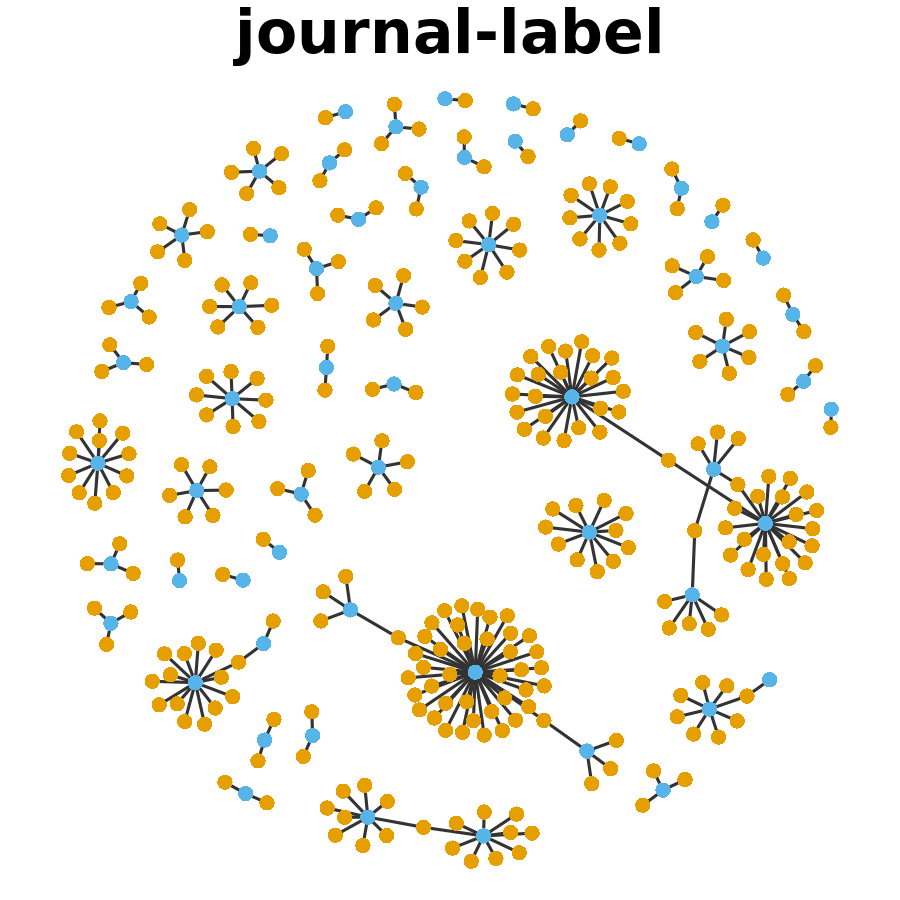
\includegraphics[width=0.33\linewidth]{ambrose_dissertation_files/figure-latex/mod-proj-1} 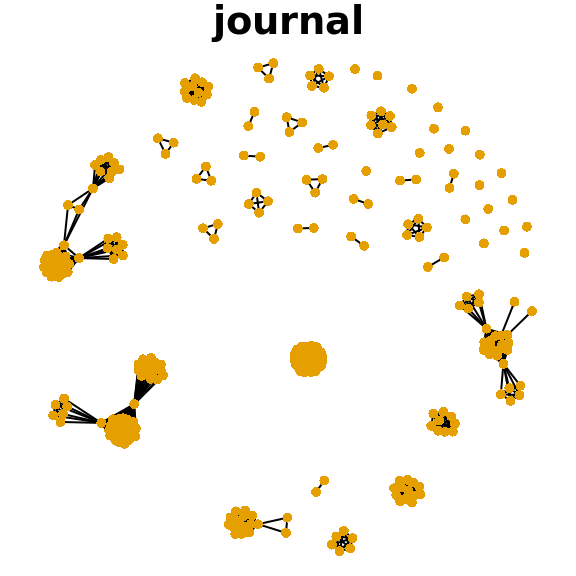
\includegraphics[width=0.33\linewidth]{ambrose_dissertation_files/figure-latex/mod-proj-2} 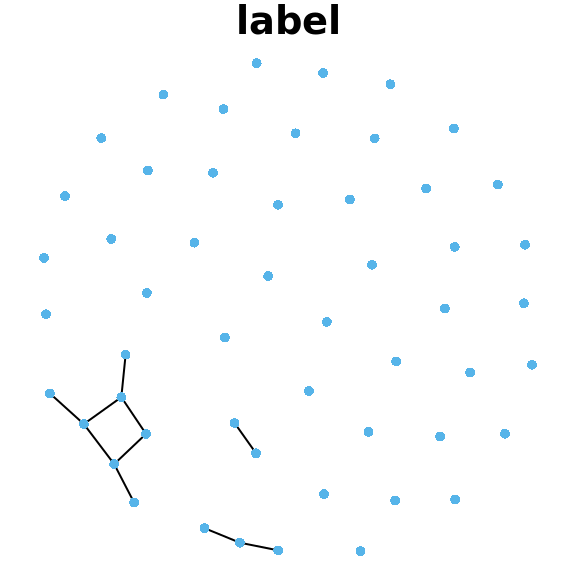
\includegraphics[width=0.33\linewidth]{ambrose_dissertation_files/figure-latex/mod-proj-3} 

}

\caption{Mode Conversion on a 300 Edge Random Sample of the JSTOR Title List Label Network}\label{fig:mod-proj}
\end{figure}

It is worth noting a few features of the unimodal projections or facets
illustrated in the second and third palens. First, unimodal projections
will always be made of up of overlapping cliques. Take the journal
facet; each journal bearing a particular label will be tied to each
other journal with the same label. Together they will form a clique, a
subnetwork of maximum density where all possible ties exist. Such
cliques grow nearly exponentially, as each additional journal with the
same label joins the clique and adds a number of ties equal to the
former size of the clique. In practice this means that very common
labels like ``Social Sciences'' can easily dominate the unimodal
projection of the network. Here the weighting of edges becomes
important; if two labels overlap because some nodes bear both labels,
then within the intersection of the two cliques the ties may be treated
as ``weighing more'' by adding the contribution of each label
separately. The exception is if the cliques overlap by only one node, in
which case they have a node but no ties in common. Nevertheless using
methods that take edge weights into account is a good way to ameliorate
the exponential influence of popular labels.

Second, though the unimodal facets of a bimodal network represent the
same data, each may have different characteristics especially in the
common case of a large population imbalance between modes. In the full
network we have 35 times as many journals as labels and each journal
sends multiple ties. This degree imbalance between the two modes may
mean that one facet is more dense than its inverse. Density is the
proportion of actual ties out of all possible ties. In Figure
\ref{fig:mod-proj} an imbalance may be observed where the journal facet
has many dense free floating or overlapping cliques and where the label
network appears to be mostly made of isolated labels save for the few
larger components. In the sampled network the journal facet is five
times more dense than the label facet. In the case of our full network,
the potential imbalance in degree distribution between facets happens to
be offset by the population imbalance itself. The densities in the full
journal and label facets are comparable, 26.2 and 27.3 percent
respectively, meaning that analysis will not merely hinge on which facet
is analyzed.

Third, unimodal projection has the effect of pruning what are sometimes
referred to as pendants, which are simply nodes with only a single tie.
. Each of the isolates in the label facet represents a larger or smaller
number of journals, which may be observed in the different sizes of the
free floating cliques of the journal facet, yet no matter their size
they supply no information about interdisciplinarity. Because the
journal facet captures both size (of cliques) and relatedness (clique
overlap) it is a better representation of the information of the
original bimodal network. Its drawback is that it is larger and more
unwieldy to analyze. The label facet offers a simpler picture of
interdisciplinarity.

\section{Network Community Detection}\label{network-community-detection}

Each facet described above will help answer a different question about
disciplinarity in the JSTOR archive as indicated by JSTOR's labeling
policy. I aim to resolve the uncertainty about which labels count as
superdisciplines and to reveal patterns of sorting not apparent in the
labels themselves. The rationale for doing this is to observe not the
choices of JSTOR coders, but the tacit judgement they likely used in
applying labels. I expect that the 79 fine grained labels bely a simpler
classification scheme of academic genres.

I will use two techniques, community detection and graph visualization,
to answer these questions. Communities are really subnetworks of high
density, or clusters. I operationalize disciplinarity as the presence of
clusters within the journal facet network. Community detection on the
journal facet will answer how many superdisciplines there are and the
size of each in terms of the number of journals belonging to it.
Visualization of the label facet will show how hard or soft are the
boundaries between disciplines and where the strongest interdisciplinary
relationships lay.

First, I use community detection to partition the JSTOR journals into
mutually exclusive disciplines. Community detection is a set of network
methods designed to expose clusters by grouping nodes together such that
they send more ties to members of their own group than they send to
members of different groups. There is a cottage industry around
developing algorithms and statistical models to learn an unobserved
community structure of a network \citep[see][ for an excellent
review]{Fortunato2016Community}. The choice of the right community
detection method is controversial especially for very large networks in
which cross-validation is difficult. Fortunately the network at hand is
small enough to validate directly which lowers the risks of choosing the
wrong method .

To wit I adopt the well-known Louvain method of community detection
based on hierarchical modularity maximization. \citep{Blondel2008Fast}
Modularity is a quality metric quantifying the tradeoff between
within-group and between-group ties. The modularity of any given
partition of a network into clusters is equal to the proportion of ties
that fall within clusters minus the expected proportion of within-group
ties if ties were distributed randomly. A division that is as good as
chance would have a modularity value of zero, a division better than
chance a value between zero and one, and a division worse than chance a
value between negative one and zero. \citep[8]{Newman2004Finding} Higher
modularity scores indicate a better sorting of the network into densely
tied clusters.

The Louvain method is a bottom-up agglomerative algorithm. The procedure
starts by assigning each node to its own community. Then, for each node,
it assigns the node to the neighbor's group that would most improve
global modularity. It repeats this until no move improves modularity.
This forms the first layer in the hierarchy. It then collapses groups
into nodes and repeats the algorithm on the condensed network, stopping
at the first level where there is no modularity improving move to make.
The first layer represents the most local, the last layer the most
global resolution of community structure.

Modularity-based methods are tried and true, and their drawbacks are
well-known. The Louvain method is not deterministic, as the outcome may
(but usually does not) depend on the ordering of the nodes in the
reassignment qeue. However Louvain has several features that recommend
it. It is computationaly fast on small to medium graphs and it is freely
available in network analysis software. It also gives a hierarchical
solution that provides the analyst with options to inspect community
structure at a range of local and global resolutions, akin to a
cartography of counties versus one of continents. Given the small size
of our network, a local resolution will not be overwhelming, so Louvain
is preferable to other methods that only offer the coarser global view.

Table \ref{tab:jclu-tab-sup} summarizes the results of applying the
Louvain method to the journal facet and taking the most localized layer
of the community structure. Learned labels are applied to the clusters
by assigning each the name of its most frequent label. Community
detection sharpens the boundaries between fields by placing each journal
unambiguously in one superdiscipline or another. This mutual exclusivity
is apparent by the sum of the given labels exceeding 100\%.

\begin{table}[!htbp] \centering 
  \caption{JSTOR Journal Counts} 
  \label{tab:jclu-tab-sup} 
\begin{tabular}{@{\extracolsep{5pt}} lrrrr} 
\\[-1.8ex]\hline 
\hline \\[-1.8ex] 
Superdiscipline & Learned & Pct & Given & GPct \\ 
\hline \\[-1.8ex] 
Social Sciences & 790 & 28.9 & 916 & 33.5 \\ 
Humanities & 664 & 24.3 & 719 & 26.3 \\ 
Area Studies & 357 & 13 & 499 & 18.2 \\ 
Science \& Mathematics & 307 & 11.2 & 360 & 13.1 \\ 
Business \& Economics & 266 & 9.7 & 285 & 10.4 \\ 
Arts & 240 & 8.8 & 293 & 10.7 \\ 
Law & 84 & 3.1 & 132 & 4.8 \\ 
Medicine \& Allied Health & 30 & 1.1 & 52 & 1.9 \\ 
Total & 2738 & 100.1 & 3256 & 118.9 \\ 
\hline \\[-1.8ex] 
\end{tabular} 
\end{table}

The first finding is that of the 79 labels these eight form the top of a
hierarchy of superdisciplines. Area Studies stands apart and is not
subsumed under either Social Sciences or Humanities. Social Sciences
journals predominate due to JSTOR's initial focus in that area, even
without counting economics among them, and Science \& Mathematics counts
for a larger than one might think. Economics stands apart from the
Social Sciences, and indeed Business \& Economics marks the transition
from the larger academic journal space to the smaller professional space
of Arts, Law, and Medicine \& Allied Health.

The given labels do overlap and we can recover a picture of
interdisciplinary by clustering and visualizing the label facet. This
facet presents a simplified view. Recall that each facet represents the
same data, the difference being whether a journal or a label is
represented as a node or an edge, and that there is a population
imbalance in favor of journals over labels. The larger the population
the easier it is to partition into a greater number of subpopulations.
Converseley, because there are far fewer labels than journals, we would
expect the clustering to be less granular for the label network than for
the journal network. In fact there is only one less cluster--Law--which
is subsumed under Social Sciences.

\section{Network Visualization}\label{network-visualization}

Figure \ref{fig:jclu-lnet} visualizations the relationships among
disciplines, where again the strength of ties is equal to the number of
journals bearing both labels. Here the label with highest number of ties
within its cluster becomes the category name of the cluster. That label
is then ommitted as a node and is instead visualized as a color coding
of its cluster, reflecting the special status of the superdiscipline
labels.

Unlike traditional graph visualizations that are designed to be pleasing
to the eye, this one is drawn according to a statistical model called a
latent position or latent space model. It starts with a simple idea that
the weight of the edges (the number of journals carrying both labels) is
a count that follows a Poisson distribution. This distribution may be
modeled by log-linear regression where the logarithm of the mean of the
distribution is a linear function of an intercept term and covariates.
What is interesting about the model is that the covariate of interest is
treated as the distance between the nodes in an unobserved or latent
space. The distance is treated as negative such that as nodes get closer
together (as the negative distance increases) the count of the edge
weight between them increases (technically the logarithm of the mean of
the count increases).

It is an elegant idea, but estimating the model is complicated. The
distances are metaphorical, and to realize them requires positing a
euclidean space in which each node has coordinates. From the coordinates
the distances can be easily caculated, but knowing which are the right
coordinates requires a complicated estimation routine based on
optimizing goodness of fit between guesses of the coordinates and the
actual count data. The estimator begins with coordinates taken from the
conventional Fruchterman Reingold layout algorithm and uses Markov Chain
Monte Carlo simulation to converge toward the positions that optimally
fit the latent space assumption \citep[See][ for details of the model,
estimation, and software]{Krivitsky2008Fitting}. Even if the estimator
does not arrive at a perfect solution it improves upon a conventional
layout in the direction of meaningful, and not just pretty, aesthetics
thereby helping the viewer to avoid artifacts and perceive real
information about the network.

Another great feature of the latent space model is that it allows
additional terms to be fit alongside the latent distances. It is
possible to control for or net out the effect of nuisance terms like any
other regression. As discussed above there is a concern about the undue
effect of popular labels. We have already tried to remove the
superdiscipline labels from the label network, preferring to represent
them as color coded categories rather than nodes. Popular labels may
still remain, however, and due to the exponential growth of ties during
downmode conversion even a handful of them will have a disproportionate
influence on the global layout of the graph.

This degree distortion can be controlled for by what is called a
sociality term, which can be thought of as a measure of a node's
popularity. A sociality term is a score for every node that if positive
means a node is more attractive and if negative means a node is actually
repulsive of ties. When viewing the positions of a latent space model
also fit with a sociality term, the space will measure relatedness
without the effects of popularity.

Figure \ref{fig:jclu-lnet} plots the results of a latent space model on
the label facet omitting superdiscipline nodes.

\begin{figure}

{\centering 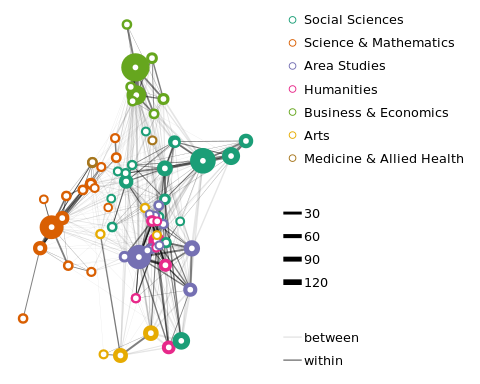
\includegraphics{ambrose_dissertation_files/figure-latex/jclu-lnet-1} 

}

\caption{Discipline Network in Latent Space. Node size represents sociality. The larger a node, the more attractive it is, and the larger a white dot within a node, the more repulsive it is.}\label{fig:jclu-lnet}
\end{figure}

Here some of the granular categories are collapsed. The humanities
includes arts, as we might expect, but also area studies, which one
might have classed with the social sciences, but which bear stronger
ties to cultural studies like music, folklore, religion, and language
and literature. Law and medicine and allied health are grouped with the
social sciences, and business and economics is maintained as separate
field due merely to the attachment of three professional
fields--development studies, management and organizational behavior, and
marketing and advertising--to their parent disciplines business and
economics (not to be confused with the separate and ommitted label
``business and economics''), which are themselves strongly tied to the
social sciences.

\begin{verbatim}
Setting the `off` event (i.e., 'plotly_doubleclick') to match the `on` event (i.e., 'plotly_click'). You can change this default via the `highlight()` function.
\end{verbatim}

\begin{figure}

{\centering \includegraphics{ambrose_dissertation_files/figure-latex/layouts-1} 

}

\caption{Fruchterman Reingold and Latent Space Layouts Compared}\label{fig:layouts}
\end{figure}

Though graph layouts are imperfect and should not be overinterpreted,
the global features of facing within clusters do indicate the
disciplines that straddle boundaries. On the border between the social
sciences and science and mathematics are the social sciences dealing
most with the physical problems of space, health, and technology. On the
edge of the humanities and social sciences are history, philosophy, and
anthropology.

\section{Social Science Journals}\label{kd-dq2}

The journals within social science cover five different subdisciplines.

\begin{table}[!htbp] \centering 
  \caption{JSTOR Social Sciences Journal Counts} 
  \label{tab:jclu-tab-sub} 
\begin{tabular}{@{\extracolsep{5pt}} lrrrr} 
\\[-1.8ex]\hline 
\hline \\[-1.8ex] 
Subdiscipline & N & Pct & Labeled & LPct \\ 
\hline \\[-1.8ex] 
Archaeology & 256 & 27.9 & 115 & 12.6 \\ 
Political Science & 219 & 23.9 & 183 & 20 \\ 
Education & 192 & 21 & 170 & 18.6 \\ 
Sociology & 160 & 17.5 & 145 & 15.8 \\ 
Anthropology & 46 & 5 & 89 & 9.7 \\ 
Population Studies & 22 & 2.4 & 27 & 2.9 \\ 
Geography & 18 & 2 & 32 & 3.5 \\ 
Transportation Studies & 3 & 0.3 & 7 & 0.8 \\ 
Total & 916 & 100 & 768 & 83.8 \\ 
\hline \\[-1.8ex] 
\end{tabular} 
\end{table}

\begin{figure}

{\centering 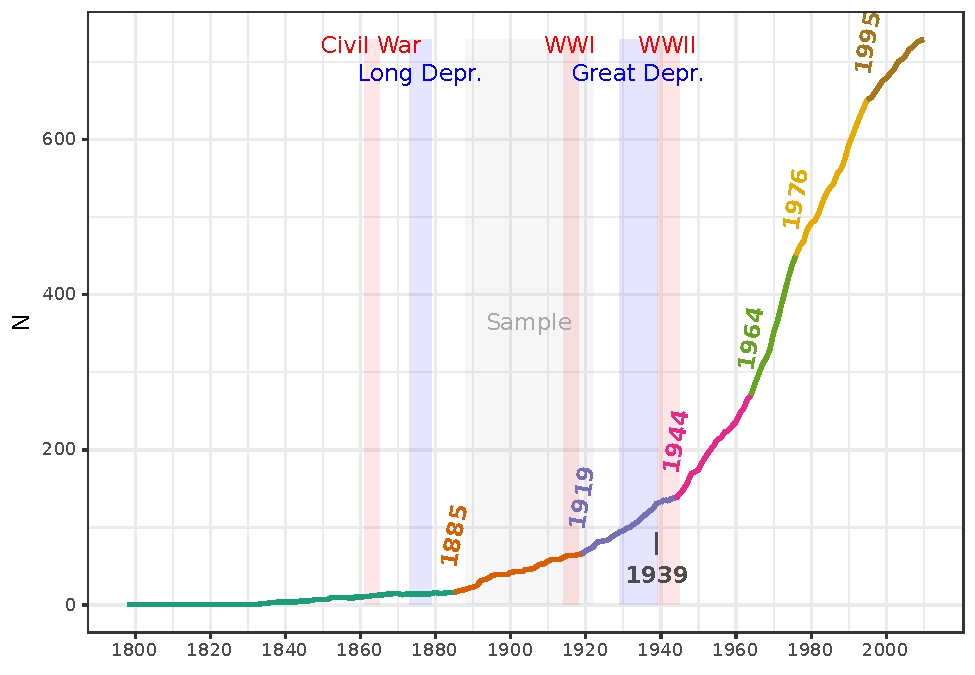
\includegraphics{ambrose_dissertation_files/figure-latex/jstorm2fig-1} 

}

\caption{Periods in the Growth of the Number of Social Science Journals in the JSTOR Archive}\label{fig:jstorm2fig}
\end{figure}

\begin{figure}

{\centering 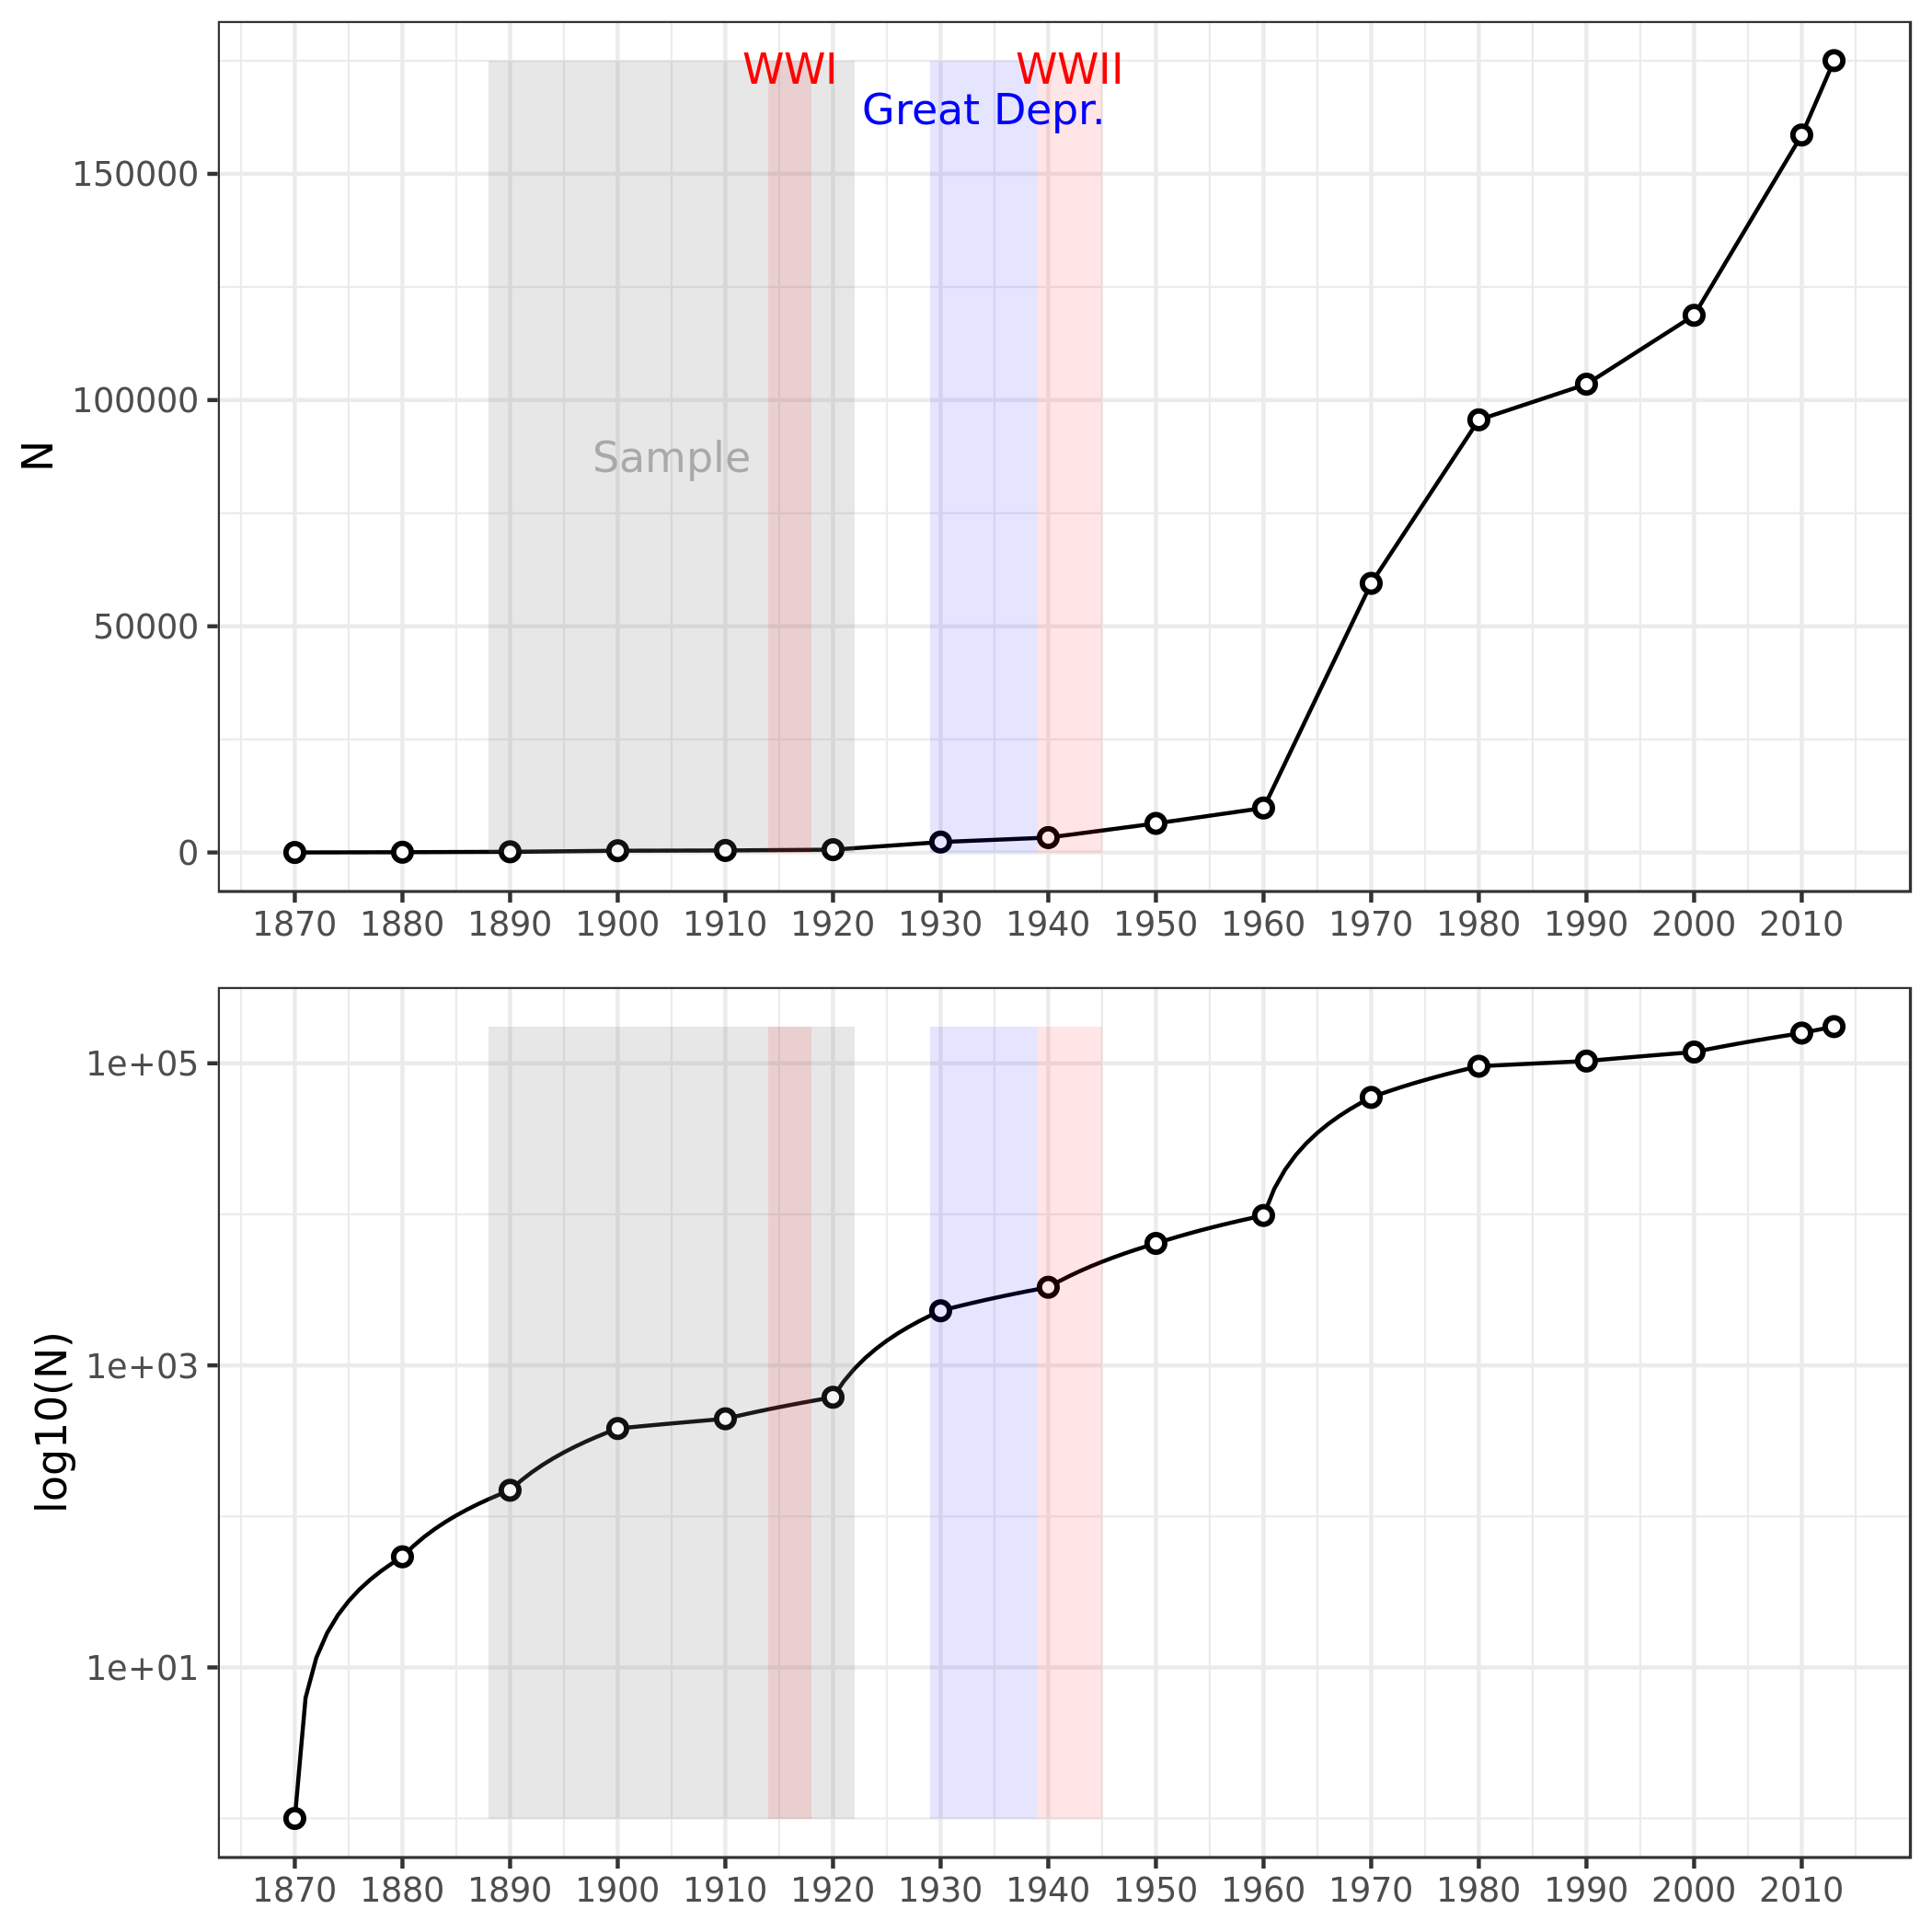
\includegraphics{ambrose_dissertation_files/figure-latex/nces2phd-1} 

}

\caption{Decennial growth in number of PhD degrees conferred in the U.S.}\label{fig:nces2phd}
\end{figure}

\begin{figure}

{\centering 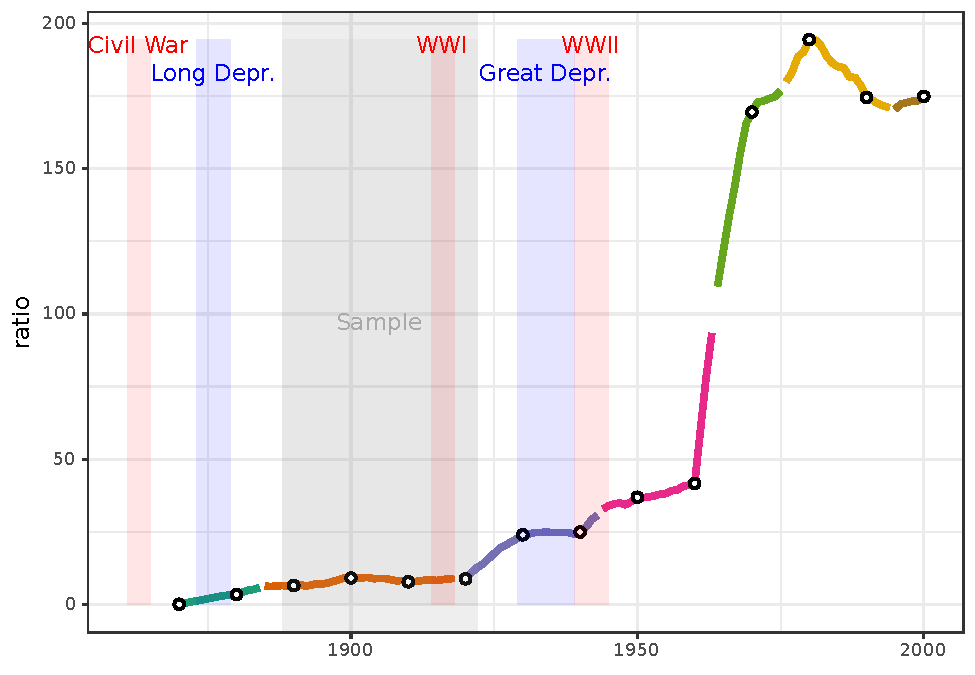
\includegraphics{ambrose_dissertation_files/figure-latex/nces/jstorm-1} 

}

\caption{Number of PhDs conferred in the United States per Social Science Journal}\label{fig:nces/jstorm}
\end{figure}

This period represents one of stable growth, as the size of the field
grows with the number of players on it. Between 1888 and 1922 there
tended to be about seven new PhDs in the U.S. for every social science
journal even as each population grew year over year. These growth
patterns begin to diverge around 1920 as a decades long acceleration of
personnel begins, relatively slowly between 1920 and 1960 at an average
acceleration rate of 22 PhDs per journal per year, and then quite
precipitously in the 1960s at an average acceleration rate of 121.

\chapter{Data}\label{kd-dd}

Every record for every journal was downloaded manually, including front
and back matter, articles, and book reviews.

\section{Sampling}\label{kd-dp1}

\begin{table}[!htbp] \centering 
  \caption{Filtering due to Data Management} 
  \label{tab:filt} 
\begin{tabular}{@{\extracolsep{5pt}} lrrrrrrr} 
\\[-1.8ex]\hline 
\hline \\[-1.8ex] 
step & doc & pag & par & sen & tok & ter & lem \\ 
\hline \\[-1.8ex] 
imported & 100 & 100 & 100 &  &  &  &  \\ 
cleaned & 99.27 & 98.21 & 67.51 &  &  &  &  \\ 
tokenized & 99.27 & 98.21 & 67.51 & 100 & 100 & 100 &  \\ 
preprocessed & 99.27 & 98.01 & 67.35 & 91.38 & 42.21 & 35.74 & 100 \\ 
sampled & 1.84 & 1.56 & 1.17 & 1.43 & 0.62 & 4.95 & 20.86 \\ 
100\\% & 5444 & 47596 & 232085 & 818183 & 19983852 & 326889 & 31963 \\ 
\hline \\[-1.8ex] 
\end{tabular} 
\end{table}

\section{Units of Analysis}\label{units-of-analysis}

Conventionally researchers feed entire documents into the construction
of term frequencies. This method treats any term in a document as being
related to any other term by the same degree. The goal of any topic
mixture model algorithm is to sift these terms into different topic
categories basically by looking for clues across documents; a topic can
be ``seen'' in a particular document to the extent that other documents
include that topic and \emph{other} topics different from the focal
article, so that the intersection of terms reveals the topic. But a much
simpler assumption to reduce the attendant noise within a document is to
merely feed lower level syntactic structures--paragraphs and
sentences--to the algorithm. We will see that doing so greatly improves
the usefulness of discovered topics.

The irony of this approach is that while topics become more clear as
documents become shorter, the assignment of any particular shorter
document to a topic is murkier due to the smaller word count.

Long documents will contribute more text to the corpus, but this is fair
as they make up more of the population of text. Thus a simple random
sample will allow better descriptive statistics. I sampled at the
paragraph level because.

\chapter{Topics}\label{kd-dp2}

The modeling objective is twofold, to sort text into categories of
similarity, and to describe the qualitative content that defines the
category membership. In this way we may operationalize the notion of
cultural meaning or cultural logic as the rules of category
classification. reduce expressions as instances of a latent category of
expression.

\section{How many topics?}\label{how-many-topics}

\begin{figure}

{\centering 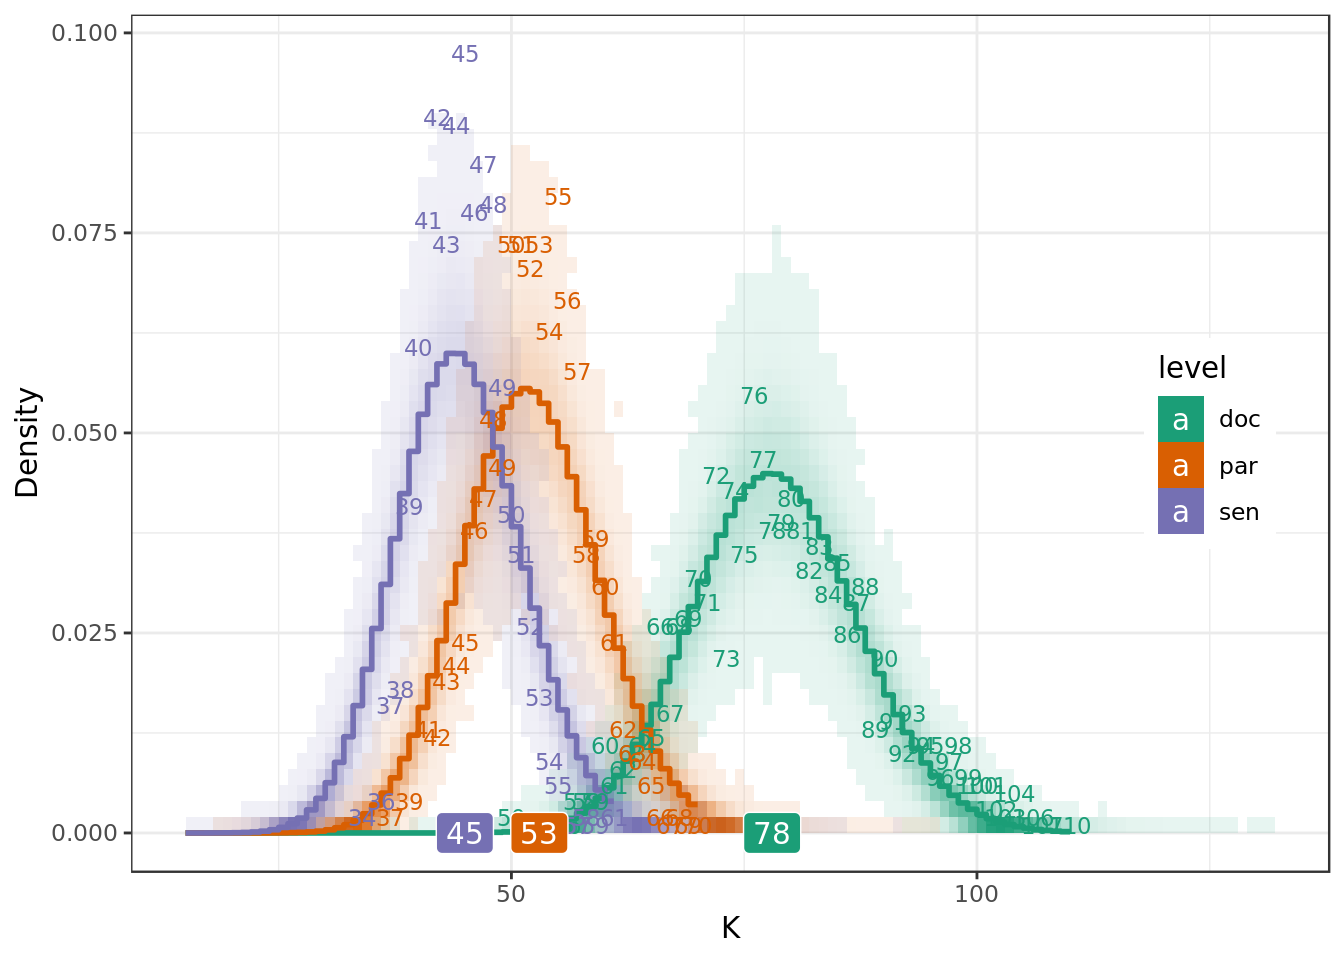
\includegraphics{ambrose_dissertation_files/figure-latex/sim-fig-1} 

}

\caption{Distribution of K by convex hull}\label{fig:sim-fig}
\end{figure}

\begin{table}[!htbp] \centering 
  \caption{Kurtosis Permutation Test} 
  \label{tab:mlk2k} 
\begin{tabular}{@{\extracolsep{5pt}} lrrrrr} 
\\[-1.8ex]\hline 
\hline \\[-1.8ex] 
level & e & se & l99 & u99 & P(e ≦ 0) \\ 
\hline \\[-1.8ex] 
doc & -0.0932 & 0.1149 & -0.3682 & 0.2252 & 0.7948 \\ 
par & -0.1125 & 0.1206 & -0.3999 & 0.2185 & 0.8257 \\ 
sen & 0.0118 & 0.2304 & -0.5078 & 0.6471 & 0.4973 \\ 
\hline \\[-1.8ex] 
\end{tabular} 
\end{table}

\begin{verbatim}
Warning: Unknown or uninitialised column: 'linetype'.
\end{verbatim}

\begin{verbatim}
Warning: Unknown or uninitialised column: 'label'.
\end{verbatim}

\begin{verbatim}
Warning: Unknown or uninitialised column: 'linetype'.
\end{verbatim}

\begin{verbatim}
Warning: Unknown or uninitialised column: 'label'.
\end{verbatim}

\begin{verbatim}
Warning: Unknown or uninitialised column: 'linetype'.
\end{verbatim}

\begin{verbatim}
Warning: Unknown or uninitialised column: 'label'.
\end{verbatim}

\begin{figure}

{\centering 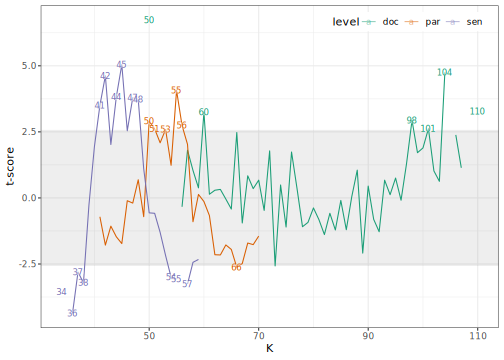
\includegraphics{ambrose_dissertation_files/figure-latex/mlk-tab-1} 

}

\caption{Significant Counts of K}\label{fig:mlk-tab}
\end{figure}

\section{Model selection}\label{model-selection}

\chapter{Web of Knowledge}\label{web-of-knowledge}

\begin{figure}

{\centering 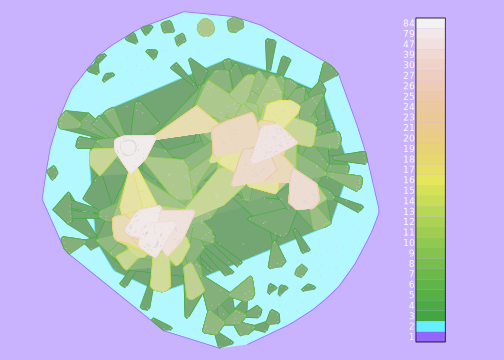
\includegraphics{ambrose_dissertation_files/figure-latex/kcc2isl-1} 

}

\caption{K-clique Community Island Plot}\label{fig:kcc2isl}
\end{figure}

\chapter{Four Fables}\label{four-fables}

What were the dominant ideas at the genesis of U.S. social research? How
would we know them if we found them? I consider two sets of approaches,
the first methodological (how?), and the second ontological (what,
why?), which will help orient us to the plan of the study. I will
briefly describe a version of the familiar distinctions among
qualitative and quantitative methods on one hand and nomathetic and
idiographic ontologies on the other. What is new is the question of
whether computational text analysis may blur the lines between these
classic social science epistemologies. In asnwering this question I will
organize some existing literature into four categories of research.

\section{\texorpdfstring{Method \emph{or} The Tortoise and the
Hare}{Method or The Tortoise and the Hare}}\label{method-or-the-tortoise-and-the-hare}

Methods are procedures for arriving at results, and they act by exposing
assumptions to empirical observations. They provide a source of
influence on arguments that breaks the circularity of their reasoning.
Methods differ in the amount of material exposed to the observer and the
speed of its exposure. The difference between human and machine learning
concerns both, but speed is especially salient.

\begin{quote}
``You may deride my awkward pace,\\
But \emph{slow and steady} wins the race.''\\
-- Robert Lloyd \citeyearpar[38]{Lloyd1762Poems}
\end{quote}

Lloyd's version of Aesop's contestants correctly describe the
consequences of haste.

First consider a humanist, a historian, a scholar with sense enough to
read primary source material. How would she proceed to conduct an
intellectual history? Slow and steady, a tortoise would identify diverse
documentary sources allowing her to collect the names of important
people and organizations and learn what she could of their biographical
facts and event timelines. She would then read the scholarship both
produced and consumed by these important actors. The identification of
ideas would be the most difficult of her tasks, not just because reading
takes time and effort (and there would be much of it), but because ideas
exist in the minds of people and leave no direct empirical trace. The
interpretation of writing in a historical context would suggest
candidate ideas; their prevalence across time and place would indicate
their historical importance. It would be tedious work requiring
intelligence and patience.

Next consider a sociologist, a computer scientist, a librarian awash in
books with no time to read them. She would identify a convenient source
and ask a computer to do the rest. Hasty, impudent, and lacking the
tortoise's fortitude and patience, a hare uses a mental prosthetic to
achieve and perhaps exceed the scale at which a humanist can consume
documentation. She learns much less than the tortoise because, whereas
people can find what they were not looking for, machines can learn only
what they are told to learn. She fails in the test of knowledge (of
course we know who wins in the end), but at least she fails quickly.

For shorthand, we can refer to these two approaches are Aesop's tortoise
and hare, the humanist mode and the computational mode.\footnote{The
  tortoise may just as well be a hammer, and the hare a steam drill, but
  for the fact that the hammer ended up losing his contest.}

\section{\texorpdfstring{Ontology \emph{or} The Fox and the
Hedgehog}{Ontology or The Fox and the Hedgehog}}\label{ontology-or-the-fox-and-the-hedgehog}

So we might learn more slowly or less quickly, but what will we be
trying to learn, and why? These concerns the question of ontology.
Ontologies are categories of being, or more simply, they are the
assumptions that answer the (usually implicit) question, ``What is
this?''. Ontologies may be descriptive categories of classification or
explanatory causal mechanisms. It is neither possible to describe nor
explain without making ontological assumptions.

\begin{quote}
``The fox knows many things,\\
but the hedgehog knows one big thing.''\\
-- Isaiah Berlin\citeyearpar[1]{Berlin1953Hedgehog}
\end{quote}

Here two of Berlin's creatures will help show two different ontological
approaches.

Consider a surveyor, an ethnographer, a data scientist. A fox believes
that the world is nothing but the facts about it. She sets out to learn
something about everything, and in so doing she tends to locate where
the action happens to be without having known it was there to begin
with. Though she can only skim for surface features, a fox's shallower
understanding of many things is usually very helpful. A fox learns where
the important, useful, or interesting things in the world are hidden.

Next consider a theorist, a statistician, a case worker. A hedgehog
learns something, but not necessarily everything, about something. They
know less than a fox, but if they are a good hedgehog then what they
know is good enough. A hedgehog experiences the world in filtered
fashion, bothering to remember only what contributes to her system or
her obsession.

So let us run Aesop's race again, but make it a three-legged race
competing in teams. And to add some purpose above crossing the finish
line, the party set an objective. The teams must gather fruit to bring
back to the table for supper. Who would win? Hare and hedgehog of
course, for they knew a big melon would provide more than their share,
which they found at a farm stand down the road. The real contest was for
second place. Hare and fox set out at once to forage, darting furiously
here and there to gather a great assortment of wild nuts and berries.
There were many mouths to feed and each morsel was small, so they had to
be dedicated to growing a larder. Tortoise and hedgehog heard tale of a
durian, the spiked and malodorous king of fruits, and thought it fit
well with hedgehog's general motif; but they did not sell them at the
country market so they walked into town looking for an importer. They
returned at sunset, durian in tow, to find hare and fox laying exhausted
atop an impressive heap of produce that hare and hedgehog had clearly
been snacking on while they idled the afternoon away. Sadly tortoise and
hare never even placed; they had thought it prudent to plant a garden of
their own and left for the seed store with no intention of returning to
the party. In a few years time they intended to be the life of the
potlach.

\section{\texorpdfstring{Plan of the Study \emph{or} A Three-Legged
Table}{Plan of the Study or A Three-Legged Table}}\label{plan-of-the-study-or-a-three-legged-table}

So in four corners of a table, three were full of different produce and
in one lay only a promise.

\begin{table}[!htbp] \centering 
  \caption{Fable Table} 
  \label{tab:fab-tab} 
\begin{tabular}{@{\extracolsep{5pt}} lrr} 
\\[-1.8ex]\hline 
\hline \\[-1.8ex] 
  & fox & hedgehog \\ 
\hline \\[-1.8ex] 
tortoise & Historian, gold standard & Historian, gold standard \\ 
hare & Historian, gold standard &  \\ 
\hline \\[-1.8ex] 
\end{tabular} 
\end{table}

\begin{quote}
``One's own consciousness dances about upon the words like a
will-o'-the-wisp.''\\
--Niklas Luhmann \citeyearpar[166]{Luhmann2002Theories}
\end{quote}

\begin{figure}

{\centering 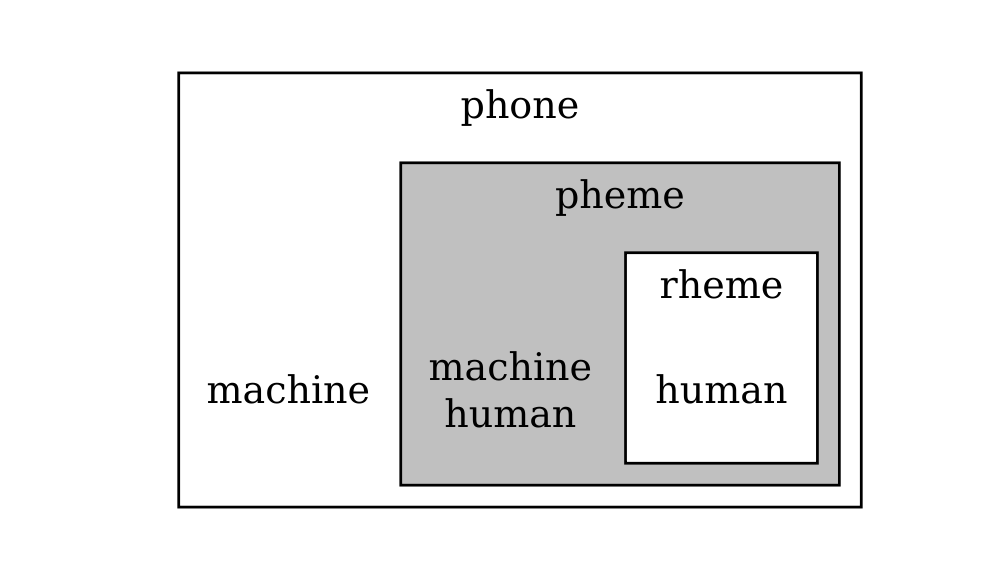
\includegraphics{ambrose_dissertation_files/figure-latex/dgr-ont-1} 

}

\caption{Ontological Approaches to Topics}\label{fig:dgr-ont}
\end{figure}

Text as thought, or as communication. Thought holds that the ideas can
be reliably interpreted, perhaps hermeneutically, to recover the mental
events or intentions of authors and readers. Ambitious. Easier is to
treat texts as communications, as messages, and worry little about their
meanings or interpretations. A study of communication is a good
foundation for the study of thought, but it is a separate task and the
one we undertake here.

\chapter{History of Ideas}\label{kd-problem}

Though the intellectual history of the social sciences begins well
before the Civil War, the current epoch of its institutional history,
the epoch of professions, becomes possible only in the postbellum
period. Before the Civil War, social research was a skilled occupation,
and individual researchers found patrons through government and civil
institutions supporting pursuits of knowledge, such as the American
Philosophical Society (APS) founded in 1743 in Philadelphia. One of the
great consequences of war was renewed federal investment in nation
building in its aftermath. Some Union congressmen saw the rebellion as a
failure of education, prompting the creation of the U.S. Department of
Education in 1867 to strengthen nation building. In the postbellum
period both anthropology and sociology develop as professions due
primarily to the growth of universities as a new context of their
activity. Without universities, social research would have remained an
occupation in need of clientele. With them, social research develops the
resources enabling relative autonomy, self reproduction, and
occupational closure, the hallmarks of a profession. This study seeks to
examine the period of transition after the Civil War from social
research as occupation to social research as profession.

\section{Antebellum Social Research
1783-1865}\label{antebellum-social-research-1783-1865}

U.S. nation building had continued since the end of the American
Revolution and had enrolled researchers in the projects of westward
expansion against native peoples, the consolidation of slave economies
against Africans, and the legitimation of the American experiment
against European detractors. These were pressing problems to the
intellectuals among government leaders at different levels, and they
worked to make investments in new knowledge to resolve them. Such new
knowledge was initially an extension of older ``theories of man'' in
theology and enlightenment natural philosophy, which had a foothold in
the private education of the American so-called natural aristocracy as
well as in urban colonial institutions like the APS serving as meeting
places for intellectual elites and scholars. After the British burned
the Library of Congress in 1914 Thomas Jefferson famously sold his
personal library to Congress to restore it, an illustration that secular
arts and sciences were produced and maintained by and under the
patronage of private elites.

The ``theory of man'' in the colonial period was that historical
progress played out along a scale from savagery to barbarism to
civilization, and that movement in the direction of progress was a
function of time and innate capacity. European societies of the Old
World had the best endowment of each, for they were very old (seen as
continuous with pre-Christian antiquity) and were lead by aristocracies
and monarchies representing the highest human capacities. Conversely
colonized peoples, and colonial societies themselves, were understood to
suffer low endowments of both, developing slowly due to their lack of
morality, reason, and aesthetics and having had less time to achieve
what little progress they could.

To gain parity with their colonial masters, the American elite altered
the theory to emphasize capacity over time. Because all men were equal,
the Americas could achieve greatness meeting or surpassing Europe given
independence and opportunity. Their masters scoffed at the idea that a
colony could ever ``catch up'' to the development of Europe, with
aristocratic families charting their roots into antiquity. American
elites, especially Southerners like Jefferson, saw themselves as
naturally superior to their countrymen, taking an aristocratic role in
their own country, but not requiring the ancient lineages qualifying
aristocracy in Europe. The values of the Declaration were egalitarian
only in this limited sense of parity across civilizations.

Egalitarianism did not mean parity within civilizations. Colonial
theologians, philosophers, and learned elites had long provided the
intellectual rationalizations of the domination of women and the
environment, and such reasoning was readily exported to the yet
unresolved problems of native tribes and African slaves. Paradoxically
egalitarian values reinforced rather than ameliorated supremacist
ideologies at home. If all men were equal, and natives (or Africans, or
women) were clearly inferior, then natives must not be men. The racism
of the Old World order in which hierarchy and domination were natural
and unproblematic, was also a consequence of egalitarian values but for
different reasons. Such racism was indeed more pernicious in America as
the concept of equality invited even more ardent ``proof'' of the
inferiority of dominated peoples.

American intellectuals knew the same logic of inferiority could be
applied to the American elite who if they could not match the rate of
progress of European society would be judged a newly diverging and
potentially inferior race of men. Though it did little to ameliorate
white male supremacist thinking, the contradictions between the
universalistic and egalitarian values expressed in the U.S. Constitution
did occasionally create grist for academic debate leading to some
investments in research critical of extant racist typologies. In Europe
scholars of comparative languages charted the supposed common origins of
European cultures and the time it had taken them to diverge. This
inspired Jefferson to patronize ethnological research on the languages
of native tribes in America. He had by 1785 amassed enough data to
appreciate their diversity, which he took as evidence that New World
cultures may be older, and therefore more developed, than commonly
assumed by colonizers.

The egalitarian-for-its-time thinking of Jefferson did not contravene
racism, but it did provide a different model of racial hierarchy, which
could be consequential for government projects. Jefferson thought that
if all men are equal, that they share the same human capacity for
progress, then native people had merely not had the time to develop and
discover progress for themselves. They could and should be taught,
especially to abandon hunting in favor of agriculture. For a brief time
in the 1840s the Virginia legislature used tax incentives and
educational programs to promote intermarriage between male settlers and
native women with the goal of accelerating the natural development of
native culture. \citep[9]{Patterson2001Social} Such experiments were
short lived, as the predictable backlash was that such mixing would risk
lowering white culture rather than elevating Indian, and genocidal and
segregationist policies won out. Thus while all racial models concluded
with the domination of natives by settlers, different models of racial
hierarchy sewed policy disputes within colonial leadership.

The role of social research then was to be in service of either
government or private political associations. Careers were made for
anthropologists in patronage relationships to generate knowledge to aid
nation builders.

\section{Postbellum Social Research
1866-1918}\label{postbellum-social-research-1866-1918}

While the roots of anthropology are as old as the republic, sociology
did not develop in earnest until after the Civil War.

\bibliography{references.bib}


\end{document}
